\section{Bucket Sort}
\subsection{Definition}
\begin{itemize}
    \item S. Sequenz (Key, Element) Entries mit Keys im Bereich [0, N-1]
    \item n: Anzahl Entries
    \item benutzt die Keys als Index in einen Hilfs-Array B von Sequenzen
    \begin{itemize}
        \item \textbf{Phase 1} Sequenz S leeren durch Verschieben jedes Entry (k, o) in sein Bucket B[k]
        \item \textbf{Phase 2} Für i = 0, ..., N - 1 verschiebe die Entries des Buckets B[i] an das Ende der Sequenz S
    \end{itemize}
\end{itemize}
\vspace{-8pt}
\begin{center}
    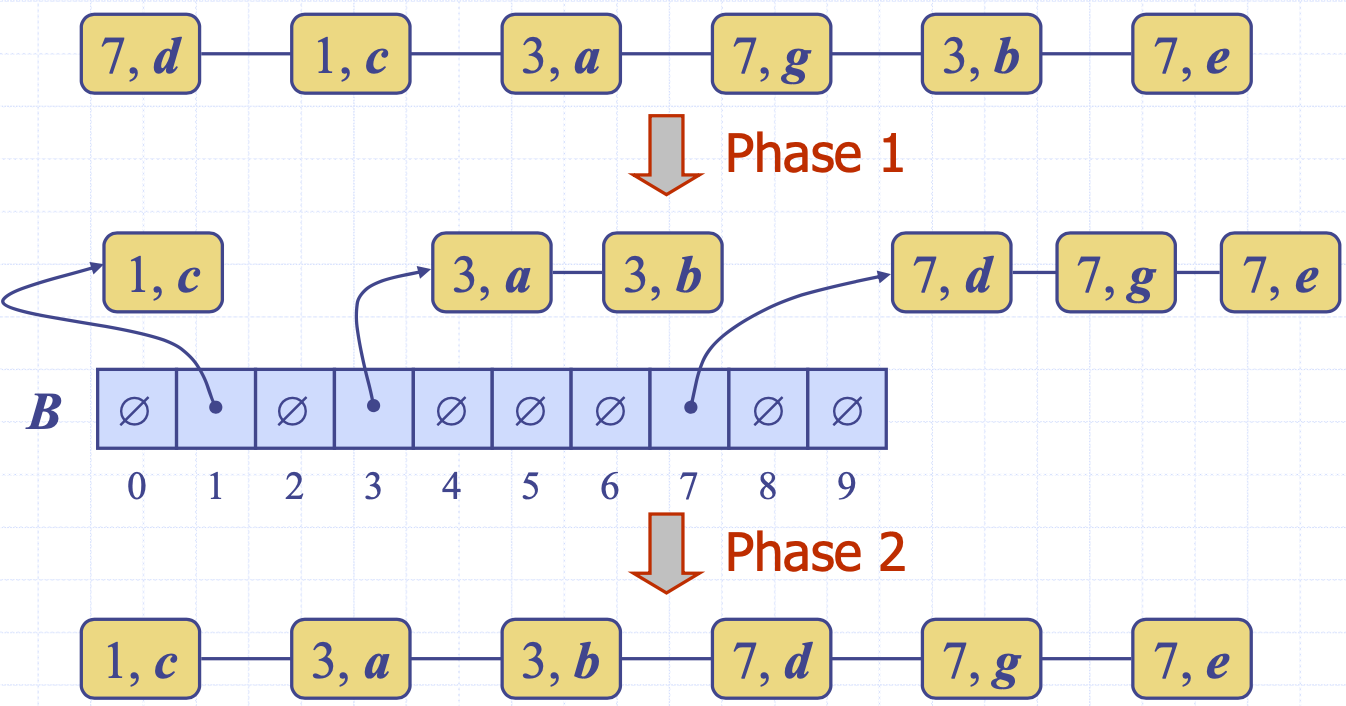
\includegraphics[scale=.22]{graphic/07 RadixSort/bucket.png}
\end{center}
\vspace{-8pt}

\subsection{Laufzeit}
\begin{itemize}
    \item Phase 1 benötigt O(n) Zeit
    \item Phase 2 benötigt O(n + N) Zeit
    \item Bucket-Sort benötigt O(n + N) Zeit
\end{itemize}

\subsection{Eigenschaften}
\subsubsection{Key}
\begin{itemize}
    \item Keys werden als Indices in einem Array benutzt und können somit nicht beliebige Objekte sein
    \item kein externer Comparator nötig
\end{itemize}
\subsubsection{Stabilität}
\begin{itemize}
    \item Die relative Ordnung von zwei Entries mit dem selben Key werden durch den Algorithmus nicht verändert
\end{itemize}

\subsubsection{Erweiterungen}
\begin{itemize}
    \item Integer Keys im Bereich [a, b]
    \item String-Keys aus einem Set D von möglichen Strings, wobei D eine konstante Grösse hat (z.B. die Namen der 50 U.S. Staaten)
\end{itemize}


\vfill
$ $
\columnbreak


\section{Lexikographische Sortierung}
\subsection{Definition}
\begin{itemize}
    \item d-Tupel ist eine Sequenz von d Keys (k1, k2, ..., kd), wobei Key ki als die i-te Dimension des Tupels bezeichnet wird
    \item Bsp: Die kartesischen Koordinaten eines Punktes im Raum sind ein 3-Tupel
    \item Die lexikographische Ordnung von zwei d-Tupels ist rekursiv definiert als:
    \begin{itemize}
        \item (x1, x2, ..., xd) < (y1, y2, ..., yd)
        \item <=>
        \item $ x1<y1 \vee  x1=y1 \wedge  (x2,...,xd) < (y2,...,yd) $
    \end{itemize}
\end{itemize}

\subsection{Laufzeit}
\begin{itemize}
    \item läuft in O(d( n + N)) Zeit
\end{itemize}

\subsection{Algorithmus}
\begin{itemize}
    \item $C_i$ der Comparator welcher zwei Tupel nach ihrer i-ten Dimension vergleicht.
    \item stableSort(S, C) sei ein stabiler Sortier-Algorithmus welcher den Comparator C benutzt
    \item Lexikographische-Sortierung sortiert eine Sequenz von d- Tupeln in lexikographischer Ordnung, indem d-mal stableSort, je einmal pro Dimension, durchgeführt wird
    \item Lexikographische-Sortierung läuft in O(d*T(n)) Zeit, wobei T(n) die Laufzeit von stableSort ist
\end{itemize}


\paragraph{Anwendung}
\begin{enumerate}
    \item Anzahl Buchstaben pro Klammer Zählen (hier 3)
    \item beginnend bei i = 3 [jeweils letzter Buchstabe]
    \item sortierung der Klammern nach Klammer[i]
    \item i - 1
    \item wiederholen bis i = 1
\end{enumerate}
\begin{center}
    Beispiel 1:\\
    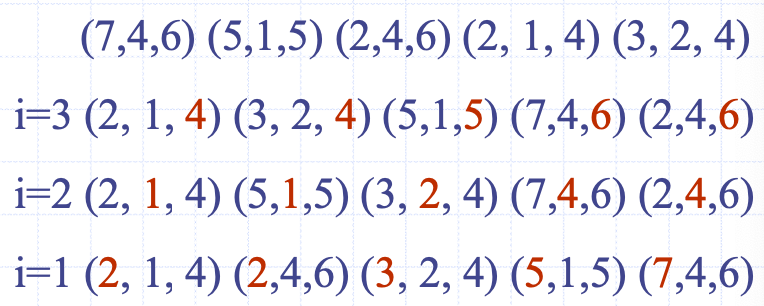
\includegraphics[scale=.3]{graphic/07 RadixSort/lexi.png}\\
    \vspace{6pt}
    Beispiel 2:\\
    \includegraphics[scale=.19]{graphic/07 RadixSort/probeprüfung_lexi.png}
\end{center}


\vfill
$ $
\columnbreak


\section{Radix Sort}
\subsection{Definition}
\begin{itemize}
    \item eine Spezialisierung des lexikographischen-Sort, welcher Bucket-Sort als stabilen Sortier- Algorithmus für jede Dimension benutzt
    \item ist anwendbar für Tupel mit Integer-Keys im Bereich [0, N - 1] in jeder Dimension i
\end{itemize}

\subsection{Laufzeit}
\begin{itemize}
    \item Beispiel: eine Sequenz von 32-Bit Integers kann in linearer Zeit sortiert werden
\end{itemize}

\subsection{für Binäre Zahlen}
\begin{itemize}
    \item Gebeben sei eine Sequenz von n b-Bit Integers:\\
    $x = x_{b - 1} ... x_1x_0$
    \item Jedes Element wird als b-Tupel von Integern im Bereich {0, 1} dargestellt. Darauf wendet man den Radix-Sort mit N = 2 an
    \item Diese Anwendung des Radix-Sort-Algorithmus läuft in O(b*n) Zeit
\end{itemize}


\vspace{-8pt}
\begin{center}
    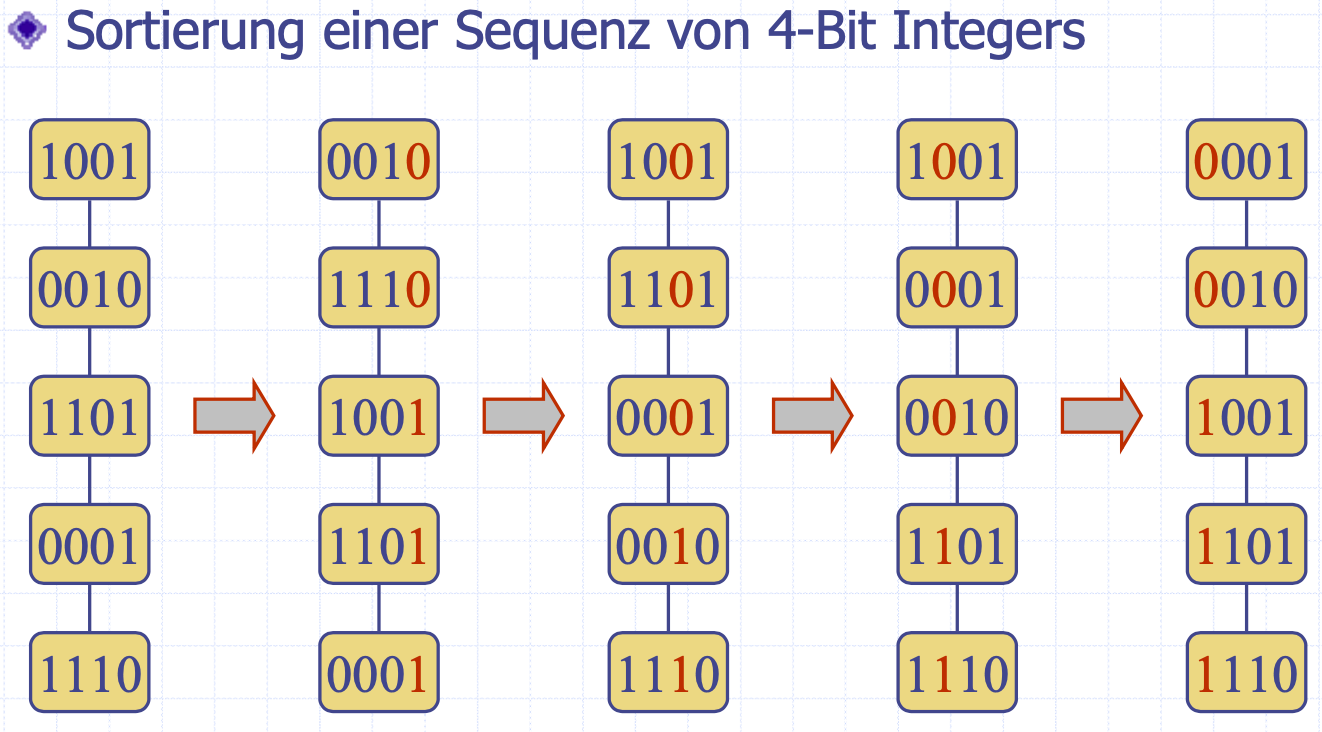
\includegraphics[scale=.2]{graphic/07 RadixSort/radix.png}
\end{center}
\vspace{-8pt}

%TODO alles nochmals schnell durchschauen, ob alles am richtigen Ort kopiert ist



\newpage